\documentclass[11pt]{article}
\usepackage[margin=0.75in]{geometry}
\usepackage{tikz}
\usepackage{array}
\usepackage{colortbl}
\usepackage{xcolor}
\usepackage{enumitem}
\usepackage{fancyhdr}
\usepackage{amsmath}
\usepackage{graphicx}

% Define colors for the gradient
\definecolor{riverblue}{RGB}{70, 130, 180}
\definecolor{col1}{RGB}{144, 238, 144}  % Light green - high yield
\definecolor{col2}{RGB}{200, 230, 150}  % Yellow-green
\definecolor{col3}{RGB}{255, 255, 180}  % Light yellow
\definecolor{col4}{RGB}{255, 220, 150}  % Light orange
\definecolor{col5}{RGB}{255, 180, 130}  % Orange - low yield
\definecolor{roadgray}{RGB}{139, 119, 101}

\pagestyle{fancy}
\fancyhf{}
\rhead{AP Statistics - Unit 3}
\lhead{Name: \underline{\hspace{2.5in}}}
\rfoot{Page \thepage}

\setlength{\parindent}{0pt}
\setlength{\parskip}{8pt}

\begin{document}

\begin{center}
{\LARGE \textbf{The Three Rivers Problem}}\\[4pt]
{\large \textit{Sampling \& Experimental Design}}
\end{center}

\vspace{0.2cm}

\textbf{Scenario:} You are an agricultural consultant hired to estimate the average corn yield of a 50-plot farm field. A \textbf{river} runs along the \textbf{left side} of the field (providing water), and a \textbf{dusty road} runs along the \textbf{right side}.

\vspace{0.3cm}

%% THE FIELD MAP %%
\begin{center}
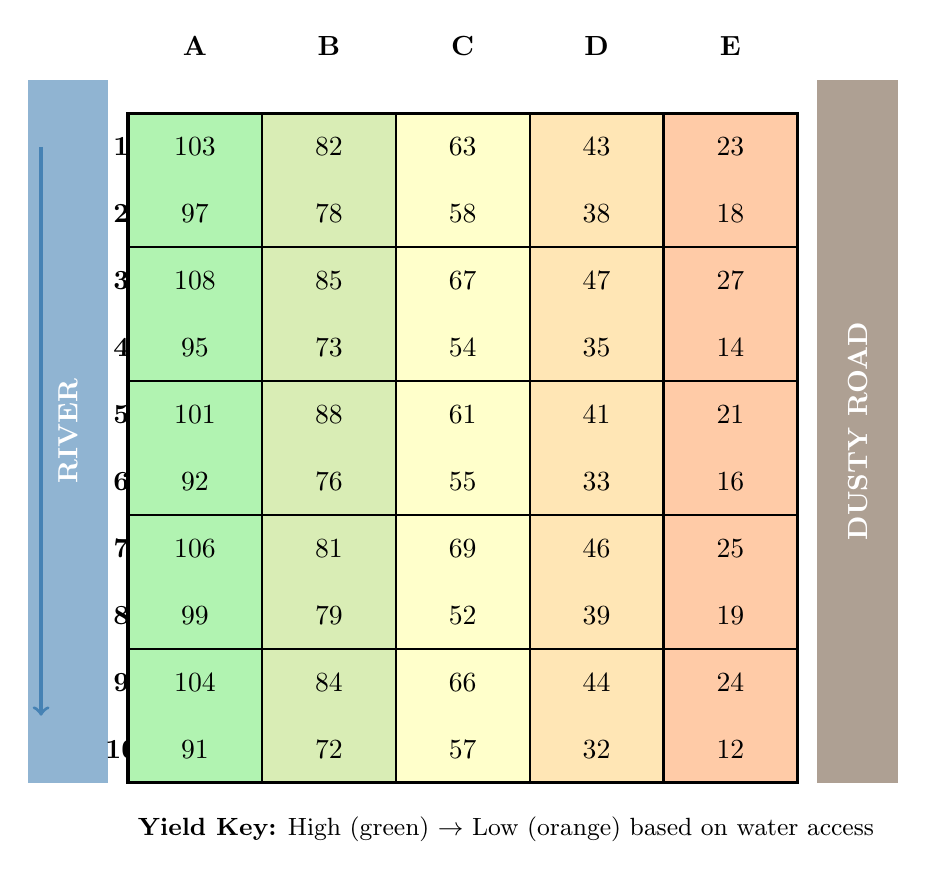
\begin{tikzpicture}[scale=0.85]
    % Draw river on left
    \fill[riverblue!60] (-1.5, 0) rectangle (-0.3, 10.5);
    \node[rotate=90, white, font=\bfseries] at (-0.9, 5.25) {RIVER};
    
    % Draw road on right
    \fill[roadgray!70] (10.3, 0) rectangle (11.5, 10.5);
    \node[rotate=90, white, font=\bfseries] at (10.9, 5.25) {DUSTY ROAD};
    
    % Column headers with color coding
    \node[font=\bfseries] at (1, 11) {A};
    \node[font=\bfseries] at (3, 11) {B};
    \node[font=\bfseries] at (5, 11) {C};
    \node[font=\bfseries] at (7, 11) {D};
    \node[font=\bfseries] at (9, 11) {E};
    
    % Row labels
    \foreach \y/\label in {0.5/10, 1.5/9, 2.5/8, 3.5/7, 4.5/6, 5.5/5, 6.5/4, 7.5/3, 8.5/2, 9.5/1} {
        \node[font=\bfseries] at (-0.1, \y) {\label};
    }
    
    % Grid cells with yields
    % Column A (River side) - High yields 90-110
    \fill[col1!70] (0,9) rectangle (2,10); \node at (1, 9.5) {103};
    \fill[col1!70] (0,8) rectangle (2,9); \node at (1, 8.5) {97};
    \fill[col1!70] (0,7) rectangle (2,8); \node at (1, 7.5) {108};
    \fill[col1!70] (0,6) rectangle (2,7); \node at (1, 6.5) {95};
    \fill[col1!70] (0,5) rectangle (2,6); \node at (1, 5.5) {101};
    \fill[col1!70] (0,4) rectangle (2,5); \node at (1, 4.5) {92};
    \fill[col1!70] (0,3) rectangle (2,4); \node at (1, 3.5) {106};
    \fill[col1!70] (0,2) rectangle (2,3); \node at (1, 2.5) {99};
    \fill[col1!70] (0,1) rectangle (2,2); \node at (1, 1.5) {104};
    \fill[col1!70] (0,0) rectangle (2,1); \node at (1, 0.5) {91};
    
    % Column B - Good yields 70-90
    \fill[col2!70] (2,9) rectangle (4,10); \node at (3, 9.5) {82};
    \fill[col2!70] (2,8) rectangle (4,9); \node at (3, 8.5) {78};
    \fill[col2!70] (2,7) rectangle (4,8); \node at (3, 7.5) {85};
    \fill[col2!70] (2,6) rectangle (4,7); \node at (3, 6.5) {73};
    \fill[col2!70] (2,5) rectangle (4,6); \node at (3, 5.5) {88};
    \fill[col2!70] (2,4) rectangle (4,5); \node at (3, 4.5) {76};
    \fill[col2!70] (2,3) rectangle (4,4); \node at (3, 3.5) {81};
    \fill[col2!70] (2,2) rectangle (4,3); \node at (3, 2.5) {79};
    \fill[col2!70] (2,1) rectangle (4,2); \node at (3, 1.5) {84};
    \fill[col2!70] (2,0) rectangle (4,1); \node at (3, 0.5) {72};
    
    % Column C - Medium yields 50-70
    \fill[col3!70] (4,9) rectangle (6,10); \node at (5, 9.5) {63};
    \fill[col3!70] (4,8) rectangle (6,9); \node at (5, 8.5) {58};
    \fill[col3!70] (4,7) rectangle (6,8); \node at (5, 7.5) {67};
    \fill[col3!70] (4,6) rectangle (6,7); \node at (5, 6.5) {54};
    \fill[col3!70] (4,5) rectangle (6,6); \node at (5, 5.5) {61};
    \fill[col3!70] (4,4) rectangle (6,5); \node at (5, 4.5) {55};
    \fill[col3!70] (4,3) rectangle (6,4); \node at (5, 3.5) {69};
    \fill[col3!70] (4,2) rectangle (6,3); \node at (5, 2.5) {52};
    \fill[col3!70] (4,1) rectangle (6,2); \node at (5, 1.5) {66};
    \fill[col3!70] (4,0) rectangle (6,1); \node at (5, 0.5) {57};
    
    % Column D - Poor yields 30-50
    \fill[col4!70] (6,9) rectangle (8,10); \node at (7, 9.5) {43};
    \fill[col4!70] (6,8) rectangle (8,9); \node at (7, 8.5) {38};
    \fill[col4!70] (6,7) rectangle (8,8); \node at (7, 7.5) {47};
    \fill[col4!70] (6,6) rectangle (8,7); \node at (7, 6.5) {35};
    \fill[col4!70] (6,5) rectangle (8,6); \node at (7, 5.5) {41};
    \fill[col4!70] (6,4) rectangle (8,5); \node at (7, 4.5) {33};
    \fill[col4!70] (6,3) rectangle (8,4); \node at (7, 3.5) {46};
    \fill[col4!70] (6,2) rectangle (8,3); \node at (7, 2.5) {39};
    \fill[col4!70] (6,1) rectangle (8,2); \node at (7, 1.5) {44};
    \fill[col4!70] (6,0) rectangle (8,1); \node at (7, 0.5) {32};
    
    % Column E (Road side) - Bad yields 10-30
    \fill[col5!70] (8,9) rectangle (10,10); \node at (9, 9.5) {23};
    \fill[col5!70] (8,8) rectangle (10,9); \node at (9, 8.5) {18};
    \fill[col5!70] (8,7) rectangle (10,8); \node at (9, 7.5) {27};
    \fill[col5!70] (8,6) rectangle (10,7); \node at (9, 6.5) {14};
    \fill[col5!70] (8,5) rectangle (10,6); \node at (9, 5.5) {21};
    \fill[col5!70] (8,4) rectangle (10,5); \node at (9, 4.5) {16};
    \fill[col5!70] (8,3) rectangle (10,4); \node at (9, 3.5) {25};
    \fill[col5!70] (8,2) rectangle (10,3); \node at (9, 2.5) {19};
    \fill[col5!70] (8,1) rectangle (10,2); \node at (9, 1.5) {24};
    \fill[col5!70] (8,0) rectangle (10,1); \node at (9, 0.5) {12};
    
    % Draw grid lines
    \draw[thick] (0,0) grid[step=2] (10,10);
    \draw[very thick] (0,0) rectangle (10,10);
    
    % Water flow arrow
    \draw[->, very thick, riverblue] (-1.3, 9.5) -- (-1.3, 1);
    
    % Legend
    \node[anchor=west, font=\small] at (0, -0.7) {\textbf{Yield Key:} High (green) $\rightarrow$ Low (orange) based on water access};
\end{tikzpicture}
\end{center}

\hrule
\vspace{0.3cm}

%% SECTION A %%
\section*{Section A: The Lazy Consultant (Convenience Sampling)}

\textbf{Scenario:} You're lazy and don't want to walk far from your truck, which is parked on the dusty road (right side of the field).

\textbf{Task:} Sample the 5 plots in \textbf{Row 1} of Column E (the rightmost column). Record the yields below and calculate the average.

\begin{center}
\begin{tabular}{|c|c|c|c|c||c|}
\hline
\textbf{E1} & \textbf{E2} & \textbf{E3} & \textbf{E4} & \textbf{E5} & \textbf{Average} \\
\hline
& & & & & \\[12pt]
\hline
\end{tabular}
\end{center}

\textbf{Reflection:} Is this estimate accurately representing the whole field? Use the terms \textbf{undercoverage} and \textbf{bias} to explain why your number is likely too low.

\vspace{0.8in}

\hrule
\vspace{0.3cm}

%% SECTION B %%
\section*{Section B: The Lottery (Simple Random Sample --- SRS)}

\textbf{Task:} Use a random number generator to select \textbf{5 unique plots} from the entire field (any location). Record the coordinates, yields, and calculate the average.

\begin{center}
\begin{tabular}{|c|c|c|c|c||c|}
\hline
\textbf{Plot 1} & \textbf{Plot 2} & \textbf{Plot 3} & \textbf{Plot 4} & \textbf{Plot 5} & \textbf{Average} \\
\hline
Coord: & Coord: & Coord: & Coord: & Coord: & \\[6pt]
\cline{1-5}
Yield: & Yield: & Yield: & Yield: & Yield: & \\[6pt]
\hline
\end{tabular}
\end{center}

\textbf{Class Comparison:} Compare your average to another group's average. Are they the same? Why might they be very different? (Think about \textbf{variation}.)

\vspace{0.8in}

\hrule
\vspace{0.3cm}

%% SECTION C %%
\section*{Section C: The Smart Consultant (Stratified Random Sample)}

\textbf{Observation:} The field looks very different near the river vs.\ the road. This suggests we should account for this structure!

\textbf{Task:} Use a \textbf{Stratified Sample}. Randomly select \textbf{one plot from each column} (A, B, C, D, and E). Record below and calculate the average.

\begin{center}
\begin{tabular}{|c|c|c|c|c||c|}
\hline
\textbf{From A} & \textbf{From B} & \textbf{From C} & \textbf{From D} & \textbf{From E} & \textbf{Average} \\
\hline
Coord: & Coord: & Coord: & Coord: & Coord: & \\[6pt]
\cline{1-5}
Yield: & Yield: & Yield: & Yield: & Yield: & \\[6pt]
\hline
\end{tabular}
\end{center}

\textbf{Analysis:} Compare this result to the SRS in Section B. Why is the Stratified method likely to give an estimate \textit{closer} to the True Mean? Use the terms \textbf{variation} and \textbf{representation}.

\vspace{0.8in}

\newpage
\fancyhead[L]{Name: \underline{\hspace{2.5in}}}

%% SECTION D %%
\section*{Section D: The Experiment (Blocking)}

\textbf{New Scenario:} A company wants to test a new ``Super-Gro'' fertilizer against the current standard fertilizer. You have 50 plots to use for this experiment.

\textbf{Question 1:} Why would a \textbf{Completely Randomized Design} (randomly assigning fertilizer to each plot) be \textit{risky} here? What confounding variable might affect your results?

\vspace{0.9in}

\textbf{Question 2:} Design a \textbf{Randomized Block Design} for this experiment.

\begin{itemize}[leftmargin=*]
    \item How would you form the \textbf{blocks}? (Hint: Look at the columns!)
    
    \vspace{0.5in}
    
    \item How would you assign treatments \textit{within} each block?
    
    \vspace{0.5in}
    
    \item Why does blocking help in this situation?
    
    \vspace{0.5in}
\end{itemize}

\textbf{Diagram:} Sketch your Randomized Block Design below. Show the blocks and indicate how treatments are assigned.

\vspace{1.5in}

\hrule
\vspace{0.3cm}

%% SYNTHESIS %%
\section*{Section E: Synthesis --- The Big Picture}

\textbf{Complete the sentence:}

\begin{center}
\fbox{\parbox{5.5in}{
\vspace{0.15in}
``We \textbf{Stratify} when we \underline{\hspace{0.6in}} to reduce \underline{\hspace{1.2in}},\\[12pt]
and we \textbf{Block} when we \underline{\hspace{0.6in}} to reduce \underline{\hspace{1.2in}}.''
\vspace{0.15in}
}}
\end{center}

\vspace{0.3cm}

\textbf{Final Reflection:} In your own words, explain the connection between stratifying (in sampling) and blocking (in experiments). Why do both methods exist?

\vspace{1in}

\newpage

%% ANSWER KEY %%
\begin{center}
{\LARGE \textbf{TEACHER ANSWER KEY}}
\end{center}

\vspace{0.3cm}

\subsection*{Field Data Summary}
\begin{itemize}
    \item \textbf{Column A (River):} 103, 97, 108, 95, 101, 92, 106, 99, 104, 91 $\rightarrow$ \textbf{Mean = 99.6}
    \item \textbf{Column B:} 82, 78, 85, 73, 88, 76, 81, 79, 84, 72 $\rightarrow$ \textbf{Mean = 79.8}
    \item \textbf{Column C:} 63, 58, 67, 54, 61, 55, 69, 52, 66, 57 $\rightarrow$ \textbf{Mean = 60.2}
    \item \textbf{Column D:} 43, 38, 47, 35, 41, 33, 46, 39, 44, 32 $\rightarrow$ \textbf{Mean = 39.8}
    \item \textbf{Column E (Road):} 23, 18, 27, 14, 21, 16, 25, 19, 24, 12 $\rightarrow$ \textbf{Mean = 19.9}
\end{itemize}

\begin{center}
\fbox{\textbf{TRUE MEAN OF ENTIRE FIELD = 59.86}}
\end{center}

\subsection*{Section A: Expected Answers}
\begin{itemize}
    \item Average of Column E Row 1-5 (E1=23, E2=18, E3=27, E4=14, E5=21): \textbf{Mean $\approx$ 20.6}
    \item This is a \textbf{biased} sample because it uses \textbf{convenience sampling}
    \item \textbf{Undercoverage}: Only plots near the road are sampled; plots near the river (with higher yields) are systematically excluded
    \item The estimate will consistently be \textbf{too low} (biased downward)
\end{itemize}

\subsection*{Section B: Expected Answers}
\begin{itemize}
    \item SRS results will \textbf{vary widely} between groups
    \item Some groups may get mostly high-yield plots, others mostly low-yield
    \item This demonstrates \textbf{high variation} in SRS estimates
    \item SRS is \textbf{unbiased} but has \textbf{high variability} when the population has distinct subgroups
\end{itemize}

\subsection*{Section C: Expected Answers}
\begin{itemize}
    \item Stratified sample should be closer to the true mean ($\approx$ 59.86) more consistently
    \item \textbf{Reduced variation}: Every sample includes representation from all yield levels
    \item \textbf{Better representation}: Guarantees coverage of the entire field's diversity
    \item Example: If selecting row 5 from each column: 101 + 88 + 61 + 41 + 21 = 312/5 = \textbf{62.4}
\end{itemize}

\subsection*{Section D: Expected Answers}
\begin{itemize}
    \item \textbf{Problem with CRD}: Water access is a \textbf{confounding variable}. By chance, Super-Gro might be assigned to more plots near the river. Higher yields would be due to water, not the fertilizer.
    \item \textbf{Blocks}: Each column (A, B, C, D, E) forms one block based on similar water access
    \item \textbf{Assignment}: Within each block of 10 plots, randomly assign 5 to Super-Gro and 5 to Standard
    \item \textbf{Benefit}: Both treatments experience similar water conditions within each block
\end{itemize}

\subsection*{Section E: Synthesis Answer}
\begin{center}
\fbox{\parbox{5.5in}{
``We \textbf{Stratify} when we \textbf{sample} to reduce \textbf{variation},\\[6pt]
and we \textbf{Block} when we \textbf{experiment} to reduce \textbf{variation}.''
}}
\end{center}

\textbf{Key insight:} Both stratifying and blocking use known sources of variation (like water access) to create more homogeneous groups. This reduces the variability in our estimates (sampling) or controls for confounding variables (experiments).

\end{document}
